\documentclass[aspectratio=169,11pt,t]{beamer}

\usepackage{fontspec}
\IfFontExistsTF{Arial}{\setmainfont{Arial}}{\setmainfont{DejaVu Sans}}
\IfFontExistsTF{Arial}{\setsansfont{Arial}}{\setsansfont{DejaVu Sans}}
\usepackage[english,russian]{babel}

\usepackage{amsmath,amssymb}
\usetheme{IPPI}
\graphicspath{{figs/}{./}}

% ---------- Math shortcuts ----------
\newcommand{\R}{\mathbb{R}}
\newcommand{\Fn}[1]{\left\|#1\right\|_F}
\newcommand{\nrm}[1]{\left\|#1\right\|}
\DeclareMathOperator{\col}{col}
\DeclareMathOperator{\tr}{tr}
\DeclareMathOperator{\spn}{span}

% ---------- Metadata (MIPT primary, IITP base chair) ----------
\title{ИССЛЕДОВАНИЕ ГЛОБАЛЬНЫХ КВАЗИНЬЮТОНОВСКИХ
МЕТОДОВ ОПТИМИЗАЦИИ ДЛЯ ЗАДАЧ ОПТИМИЗАЦИИ И
ВАРИАЦИОННЫХ НЕРАВЕНСТВ}
\author{Можаев Роман Михайлович}
\supervisor{Камзолов Дмитрий Игоревич, канд.\,физ.-мат.\,наук}
\organization{%
  Московский физико-технический институт\\
  (национальный исследовательский университет)\\
  Физтех-школа прикладной математики и информатики\\
  Кафедра проблем передачи информации и анализа данных\\
  \textit{(базовая кафедра ИППИ РАН)}%
}
\city{Москва, 2026}
\defensedate{16.06.2026}
\orglogo{mipt_logo.png}

\begin{document}

% ===================== ТИТУЛ =====================
\begin{frame}[plain,noframenumbering]
  \titlepage
\end{frame}

% ===================== ПЛАН =====================
% Говорить: коротко перечислить, не задерживаться (15–20 сек).
\begin{frame}{План доклада}
  \begin{enumerate}
    \item Мотивация, цель и предмет
    \item Мультисекущий Бройден: точная теорема об ограниченной деградации
    \item Limited-memory вариант L-PB
    \item Симметричный аналог SS-U для оптимизации
    \item Приложение к вариационным неравенствам
    \item Выводы
  \end{enumerate}
\end{frame}

% ===================== МОТИВАЦИЯ 1 =====================
% Говорить: приложения + «при больших n решает стоимость итерации». Ньютон и проблему — на след. слайде.
\begin{frame}{Мотивация}
Базовая задача вычислительной математики — решить нелинейную систему
\[ F(x)=0,\quad F\colon\R^n\to\R^n,\qquad\text{или найти}\quad \min_{x\in\R^n} f(x). \]
Такие задачи возникают всюду: дискретизация дифференциальных уравнений, обучение
моделей, поиск равновесий в играх и экономике (вариационные неравенства).

\medskip
Замкнутого решения в общем случае нет — строится последовательность приближений
\(x_0,x_1,x_2,\ldots\). При больших \(n\) решающей становится \emph{стоимость одной
итерации}: вычислять производную на каждом шаге слишком дорого.
\end{frame}

% ===================== МОТИВАЦИЯ 2 =====================
% Говорить: Ньютон точен, но дорог; QN заменяет якобиан накопленной матрицей;
% классические обновления чувствительны к старту — это и есть проблема.
\begin{frame}{От Ньютона к квазиньютоновским методам}
Метод Ньютона строит линейную модель \(F\) в \(x_k\):
\[ J_F(x_k)\,s_k=-F(x_k),\qquad x_{k+1}=x_k+s_k. \]
Трудность: на каждой итерации нужен якобиан \(J_F(x_k)\) и решение линейной системы —
дорого, а часто \(J_F\) и вовсе недоступен.

\medskip
\textbf{Квазиньютоновская идея.} Заменить \(J_F(x_k)\) матрицей \(B_k\), строящейся
по уже полученным данным (без вычисления производных):
\[ B_k\,s_k=-F(x_k),\qquad x_{k+1}=x_k+s_k. \]
\end{frame}

% ===================== МОТИВАЦИЯ 2 (часть 2) =====================
\begin{frame}{От Ньютона к квазиньютоновским методам}
\textbf{Проблема.} Классические обновления (Бройден, SR1, BFGS) без глобализации
сходятся лишь \emph{локально} и чувствительны к старту.

\medskip
Локальную сходимость выводят из \emph{ограниченной деградации} (bounded deterioration)
— контроля роста ошибки аппроксимации
\[ E_k=B_k-J^*,\qquad J^*=J_F(x^*). \]
Именно эту оценку работа и уточняет: окно прошлых шагов контролирует деградацию.
\par\medskip
{\scriptsize Локальная сверхлинейная сходимость: Broyden, Dennis, Moré (1973);
необходимость глобализации (line search): Griewank (1986).}
\end{frame}

% ===================== ПРОБЛЕМА — ЧИСЛЕННО (4b) =====================
% Говорить (~35 сек, можно сжать/пропустить): иллюстрация ЦИТИРУЕМОГО факта на
% стандартном тесте MGH (не свой пример); близко — сходимость, далеко — расходимость.
\begin{frame}{Проблема численно: чувствительность к старту}
\centering
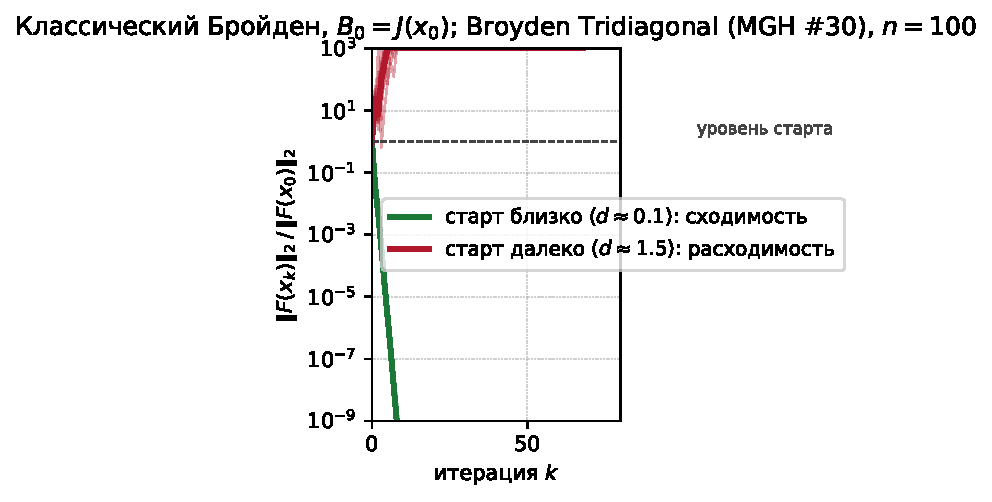
\includegraphics[width=0.72\textwidth]{fig_motiv_start_sensitivity.pdf}
\par
{\footnotesize\raggedright
Классический Бройден, \(B_0=J_F(x_0)\); тест Broyden Tridiagonal (Moré–Garbow–Hillstrom
1981, \#30), \(n=100\). Близкий старт сходится сверхлинейно, далёкий — расходится:
конечная \emph{область сходимости}, без глобализации сходимость не гарантирована
(документировано: Griewank 1986).\par}
\end{frame}

% ===================== ЦЕЛЬ И ПРЕДМЕТ =====================
% Говорить: смысл слова «глобальные» проговаривается УСТНО (сноску убрали);
% постановка перед идеей — без превью результатов (вклад разбирается по ходу + в Заключении).
\begin{frame}{Цель и предмет исследования}
\textbf{Цель.} Развить количественный анализ ошибки аппроксимации якобиана
\(E_k=B_k-J^*\) в квазиньютоновских методах с памятью прошлых шагов — для систем
\(F(x)=0\), гладкой оптимизации и вариационных неравенств (ВН).

\medskip
\textbf{Предмет.} Квазиньютоновские обновления \(B_k\), сохраняющие \(p\) прошлых
секущих условий \(B_{k+1}s_j=y_j\) и порождающие расширенный (ранг \(p{+}1\)) проектор
ограниченной деградации (bounded deterioration).
\end{frame}

% ===================== МУЛЬТИСЕКУЩАЯ ИДЕЯ (мост гл.1) =====================
\begin{frame}{Мультисекущая идея}
Шаг \(s_k\) даёт информацию \(y_k=F(x_{k+1})-F(x_k)=\bar J_k\,s_k\approx J^*s_k\)
(\(\bar J_k\) — средний якобиан). \emph{Секущее условие}: \(B_{k+1}\) воспроизводит \(y_k\) вдоль шага:
\[ B_{k+1}s_k=y_k,\qquad s_k=x_{k+1}-x_k. \]
\textbf{Классический Бройден} держит \emph{одно} условие
\(B_{k+1}=\arg\min\{\Fn{B-B_k}:Bs_k=y_k\}\) — проектор ранга 1 на \(\spn s_k\).

\textbf{Мультисекущий Бройден.} Окно \(S_p=[\,s_k\mid s_{k-1}\mid\cdots\mid s_{k-p}\,]\),
\(Y_p\) аналогично, \(G_p=S_p^\top S_p\):
\[ B_{k+1}=\arg\min\{\Fn{B-B_k}:\ B S_p=Y_p\}
        =B_k+(Y_p-B_kS_p)\,G_p^{-1}S_p^\top. \]
Держит \(p{+}1\) секущих (\(p=0\) — классический Бройден).
\smallskip
{\scriptsize Требовать все накопленные секущие сразу численно неустойчиво (Griewank 2012): почти линейно зависимые шаги \(\Rightarrow\) \(G_p\) почти
вырождена \(\Rightarrow\) \(G_p^{-1}\) усиливает ошибки.}
\end{frame}

% ===================== ТЕОРЕМА 2.10 (ЦЕНТР) =====================
% Говорить (центральный слайд, ~1.5 мин): «равенство, а не неравенство»;
% «константа не зависит от n — это и открывает дорогу к limited-memory».
\begin{frame}{Теорема об ограниченной деградации (гл.~2)}
\(E_k=B_k-J^*\), \(\Pi_k=S_pG_p^{-1}S_p^\top\) — проектор на \(\col(S_p)\),
\(\rho_k\) — расстояние до корня.
\smallskip

{\small Прежде (Гэй–Шнабель, 1978, Th.~4.2; ранг-1, \(p=0\)) — лишь оценка сверху
\(\Fn{E_{k+1}}\le\Fn{E_k}+O(\rho_k)\) без явной константы. Здесь (ранг \(p{+}1\)):}

\medskip
\textbf{(a) Точное равенство:}\quad
\(\Fn{E_{k+1}}^2=\Fn{E_k}^2-\Fn{E_k\Pi_k}^2+\Delta_k.\)

\medskip
\textbf{(b) Bounded deterioration:}
\[ \Fn{E_{k+1}}^2\le\Fn{E_k}^2-\Fn{E_k\Pi_k}^2+C_{\mathrm{PB}}^2\,\rho_k^2. \]
\end{frame}

% ===================== ТЕОРЕМА 2.10 (часть 2) =====================
\begin{frame}{Теорема об ограниченной деградации (гл.~2)}
\[ \Fn{E_{k+1}}^2\le\Fn{E_k}^2-\Fn{E_k\Pi_k}^2+C_{\mathrm{PB}}^2\,\rho_k^2. \]
\begin{itemize}\setlength{\itemsep}{8pt}
  \item \(C_{\mathrm{PB}}=L\big(1+\tfrac{C_s}{2}\big)\sqrt{p+1}\,\kappa_p\)
        (\(\kappa_p=\kappa(S_p)\)) — зависит от окна, \textbf{не от \(n\)}.
  \item \(\Fn{E_k\Pi_k}^2\ge\nrm{E_ks_k}^2/\nrm{s_k}^2\): стягивание на всём
        \((p{+}1)\)-мерном окне, не на прямой \(s_k\).
  \item \textbf{Зачем:} BD \(\Rightarrow\) локальная сходимость;
        \(n\)-независимая \(C_{\mathrm{PB}}\) \(\Rightarrow\) L-PB.
\end{itemize}
\end{frame}

% ===================== СЛЕДСТВИЕ 2.12 =====================
\begin{frame}{Следствие: контроль ошибки на подпространстве}
\[ \Fn{E_{k+1}S_p}\ \le\ L\Big(1+\tfrac{C_s}{2}\Big)\sqrt{p+1}\,\sigma_{\max}(S_p)\,\rho_k. \]
\(B_{k+1}\) аппроксимирует \(J^*\) на \emph{всём} \(\col(S_p)\) с точностью \(O(\rho_k)\),
определяемой \emph{расстоянием до корня} \(\rho_k\), а \emph{не} накопленной ошибкой \(\Fn{E_k}\).

\medskip
\textbf{Структурное преимущество.} У классического Бройдена безусловный
\(O(\rho_k)\)-контроль есть лишь вдоль одномерного направления \(s_k\); на остальном
подпространстве ошибка определяется глобальной историей итераций.

\medskip
\textbf{Зачем нужно.} Эта подпространственная оценка подставляется в роль неточности
\(\delta\) в методе 2-го порядка для ВН (гл.~4, Утв.~4.1).
\end{frame}

% ===================== L-PB =====================
\begin{frame}{Limited-memory вариант L-PB}
Плотная \(B_k\in\R^{n\times n}\): \(O(n^2)\) памяти, \(O(n^3)\) флопс на шаг
(\(n=10^5\Rightarrow\approx80\) ГБ) — неприменимо.

\medskip
\textbf{Почему ранг-1.} Projected Broyden обновляет \emph{обратную} матрицу рангом 1
(формула Шермана–Моррисона) с секуще-сохраняющим \(v_k=S_pG_p^{-1}e_1\): из
\(v_k^\top s_k=1\) и \(v_k\perp s_{k-1},\dots,s_{k-p}\) шаг \emph{добавляет} текущую
секущую, сохраняя \(p\) прошлых.
\[ H_{k+1}=H_k+\frac{(s_k-H_ky_k)\,v_k^\top H_k}{v_k^\top H_ky_k},\qquad H_{k+1}y_k=s_k. \]
\end{frame}

% ===================== L-PB (часть 2) =====================
\begin{frame}{Limited-memory вариант L-PB}
\textbf{Limited memory.} \(H_k\) не формируется: окно из \(m\) троек \((s_j,y_j,v_j)\),
применение \(H_kg\) — рекурсия типа L-BFGS (там пары, здесь тройки; \(p_{\max}=0\) даёт
L-Broyden). Стоимость \(\mathcal{M}=O(nm)\) памяти, \(O(nm^2)\) флопс/итерацию.

\medskip
\begin{itemize}\setlength{\itemsep}{8pt}
  \item \(p=\min(p_{\max},k)\); при \(m\ge p_{\max}{+}1\) выполнено L-PB \(\equiv\) плотный PB
        на последних \(p_{\max}{+}1\) секущих (Утв.~2.1).
  \item \(\Rightarrow\) Теорема 2.10 переносится \emph{дословно}, та же
        \(C_{\mathrm{PB}}\propto\kappa_p\) (не от \(n\)): экономия памяти не стоит ничего
        в теории.
\end{itemize}
\end{frame}

% ===================== ЧИСЛЕННОСТЬ ГЛ.2 — рис.1 =====================
% Говорить: главный месседж — «ошибка ограничена, но Бройден всё равно не сходится;
% окно переводит в режим сверхлинейной сходимости».
\begin{frame}{Численный результат: Discrete BVP (\(n=100\))}
\centering
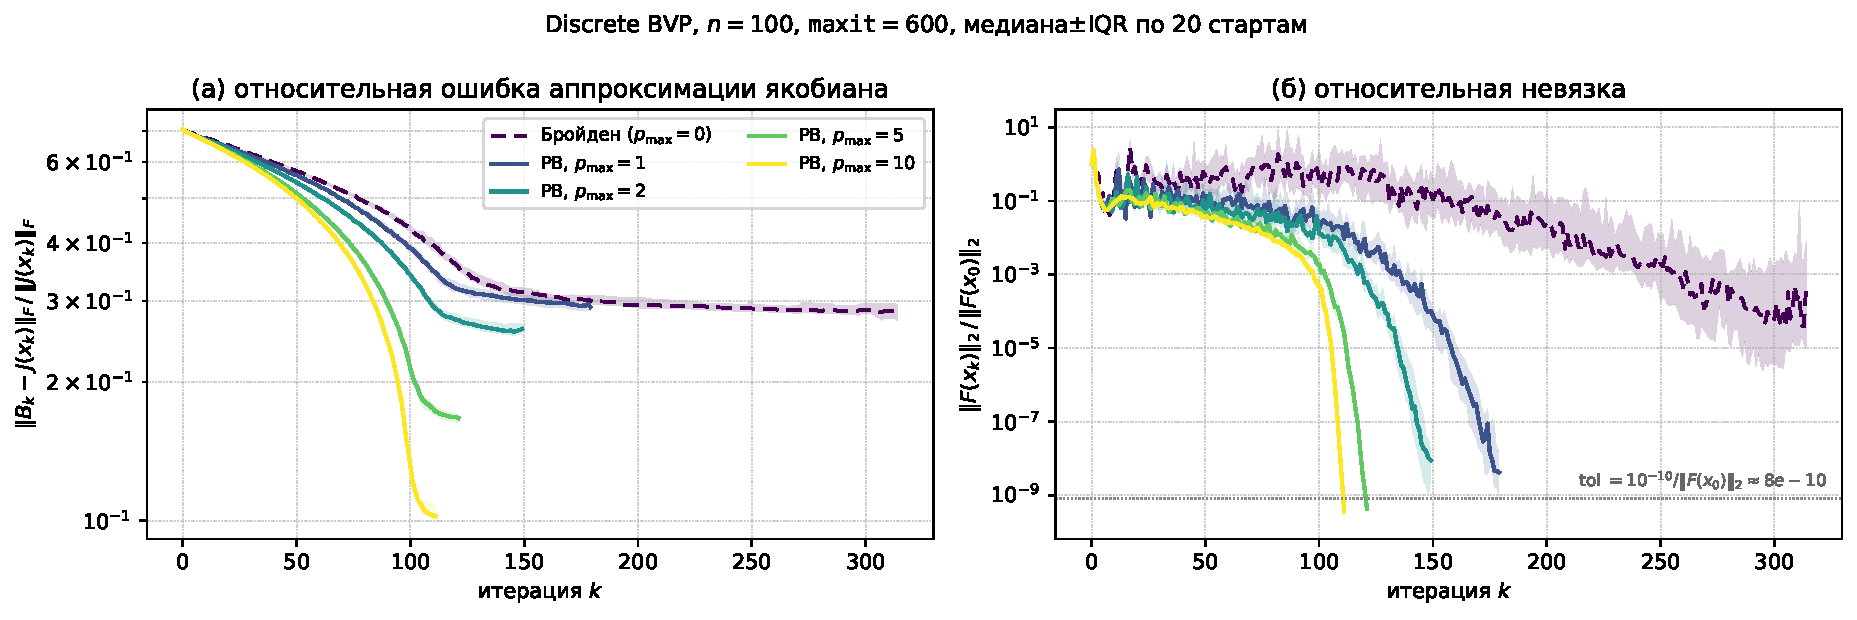
\includegraphics[width=0.92\textwidth]{fig_sp_broyden_jacerr.pdf}
\par\smallskip
{\footnotesize\raggedright
Классический Бройден (\(p_{\max}=0\)) \textbf{не сходится} ни на одном из 20 стартов;
PB при \(p_{\max}\ge1\) устойчиво сходится на всех. Расширение окна переводит метод из
режима «ошибка ограничена, сходимости нет» в режим сверхлинейной сходимости.\par}
\end{frame}

% ===================== ЧИСЛЕННОСТЬ ГЛ.2 — рис.2 (high-dim) =====================
\begin{frame}{L-PB в высокой размерности: Broyden Banded}
\centering
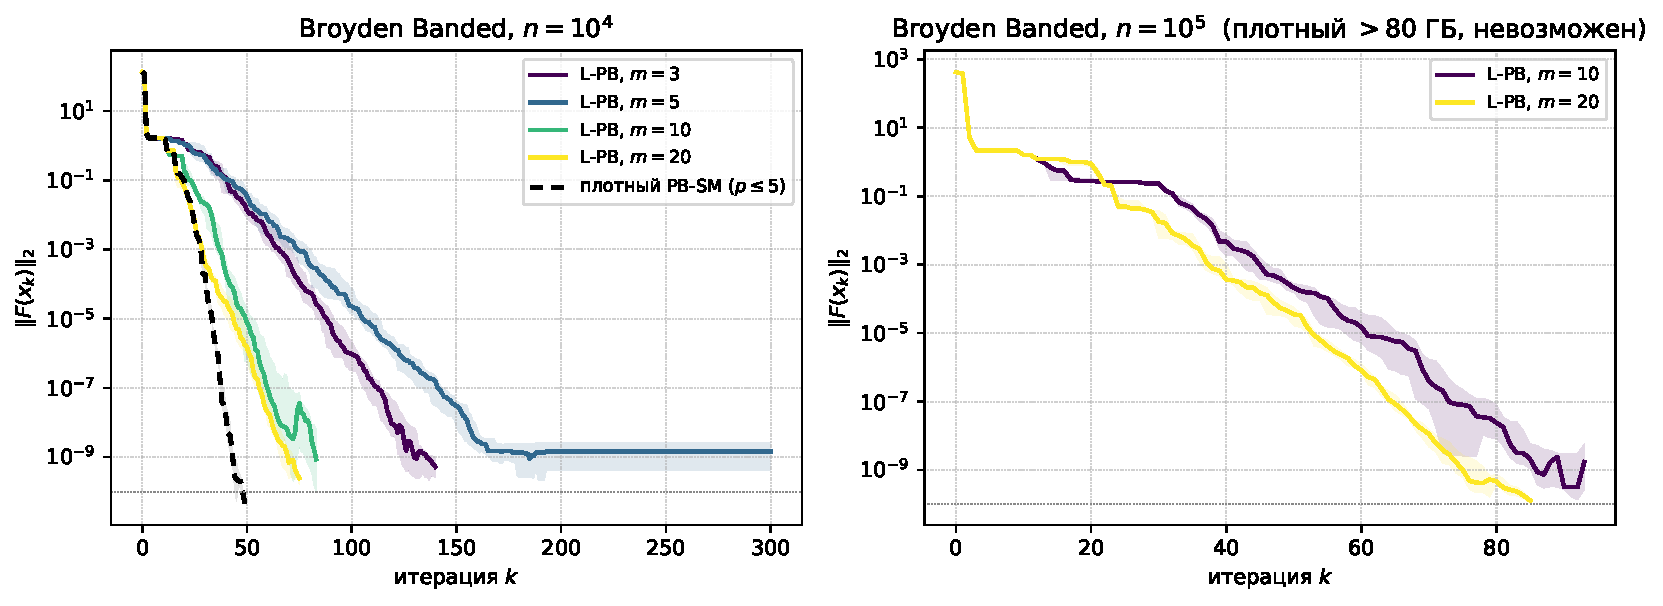
\includegraphics[width=0.86\textwidth]{fig_highdim_conv.pdf}
\par\smallskip
{\footnotesize\raggedright
При \(n=10^5\) плотная форма требует \(\approx80\) ГБ и неприменима; L-PB сходится за
число итераций, \emph{не растущее} с \(n\). Деградация по глубине окна \(m\) умеренная и
согласуется с теорией (ср. L-BFGS).\par}
\end{frame}

% ===================== SS-U: КОНСТРУКЦИЯ =====================
\begin{frame}{Симметричный случай: конструкция SS-U}
\textbf{Зачем симметрия.} В оптимизации \(B_k\) приближает \emph{симметричный} гессиан
\(\nabla^2 f\): симметричная \(B_k\) отвечает корректной квадратичной модели.

\medskip
\textbf{Несовместимость (Лемма 3.1, Шнабель).} В общем положении нельзя одновременно
сохранить симметрию \(B_{k+1}=B_{k+1}^\top\) и несколько секущих условий — симметрия и
мультисекущность конфликтуют.

\medskip
\textbf{Идея SS-U.} Взять базовое \emph{симметричное} обновление, точно держащее
\emph{текущую} секущую, и добавить поправку на
согласование с \emph{прошлыми} секущими — не разрушая ни симметрию, ни \(B_{k+1}s_k=y_k\).
\end{frame}

% ===================== SS-U: КОНСТРУКЦИЯ (часть 2) =====================
\begin{frame}{Симметричный случай: конструкция SS-U}
\small
База \(B_k'=\mathcal{U}(B_k,s_k,y_k)\) (SR1/PSB; \(B_k's_k=y_k\)), невязка на окне
\(R_k'=B_k'S_p-Y_p\) (текущий столбец \(B_k's_k-y_k=0\)). Ранг-1 коррекция \(\perp s_k\)
(тогда \(B_{k+1}s_k=y_k\) и симметрия сохраняются):
\[ (\sigma_k^\star,u_k^\star)\in\arg\min_{u\perp s_k,\,\nrm{u}=1,\,\sigma}
   \Fn{R_k'+\sigma\,uu^\top S_p},\qquad B_{k+1}=B_k'+\sigma_k^\star\,u_k^\star u_k^{\star\top}. \]

\textbf{Как находить \((u_k^\star,\sigma_k^\star)\) (Лемма 3.7).} При фиксированном \(u\)
минимум по \(\sigma\) точный: \(\sigma_k^\star(u)=-\dfrac{u^\top M_k'\,u}{\nrm{S_p^\top u}^2}\),\ \
\(M_k'=\tfrac12(R_k'S_p^\top+S_pR_k'^{\top})\). Минимизация по \(u\) — задача без
замкнутой формы, поэтому используется \emph{гибрид}:
\[ u_k^\star=\text{ведущий собственный вектор }P_kM_k'P_k\big|_{s_k^\perp},\ \
   P_k=I-\hat s_k\hat s_k^\top;\qquad \sigma_k^\star=\sigma_k^\star(u_k^\star). \]

\smallskip
\textbf{Свойства (Теорема 3.8):} \(B_{k+1}s_k=y_k\), симметрия, ранг \(1\); невязка прошлых
секущих убывает на \((\sigma_k^\star)^2\nrm{S_p^\top u_k^\star}^2\).
\end{frame}

% ===================== SS-U: СХОДИМОСТЬ =====================
\begin{frame}{Сходимость SS-U}
\textbf{Лемма 3.12 (композитное bounded deterioration).} При липшицевом гессиане и
достаточной близости старта:
\[ \Fn{E_{k+1}}^2\le\Fn{E_k}^2-\frac{\nrm{E_ks_k}^2}{\nrm{s_k}^2}+\beta_k,
   \qquad \sum_{k}\beta_k<\infty, \]
Здесь \(\beta_k=\beta_k^{(\mathcal U)}+\beta_k^{(SS)}\ge0\) — композитная деградация за шаг:
\[ \beta_k^{(\mathcal U)}=c_{\mathcal U}L_H\alpha_k\ \ (\text{база }\mathcal U),\qquad
   \beta_k^{(SS)}=2|\sigma_k^\star|\,\Fn{E_k'}+(\sigma_k^\star)^2\ \ (\text{ранг-1 коррекция}), \]
\(\alpha_k\sim\) расстояние до \(x^*\), \(E_k'=B_k'-J^*\). 
\end{frame}

% ===================== SS-U: СХОДИМОСТЬ (часть 2) =====================
\begin{frame}{Сходимость SS-U}
Просуммируем неравенство
леммы~3.12 (\(\Fn{E_{N+1}}^2\ge0\), \(\sum_k\beta_k<\infty\)):
\[ \sum_k\frac{\nrm{E_ks_k}^2}{\nrm{s_k}^2}<\infty
   \quad\Rightarrow\quad \frac{\nrm{E_ks_k}}{\nrm{s_k}}\to0. \]
\(\Rightarrow\) условие Денниса–Море выполняется.

\medskip
\textbf{Теорема 3.9 (условная Q-сверхлинейность).} При невырожденном пределе и
допустимости полного шага:
\[ \underbrace{\frac{\nrm{(B_k-J^*)s_k}}{\nrm{s_k}}\xrightarrow[k\to\infty]{}0}_{\text{условие Денниса–Море}}
   \quad\Rightarrow\quad \frac{\nrm{x_{k+1}-x^*}}{\nrm{x_k-x^*}}\to 0. \]
\end{frame}

% ===================== ЧИСЛЕННОСТЬ ГЛ.3 — рис.4 =====================
% Говорить ЧЕСТНО: SS спасает деградирующее обновление; где деградации нет (SR1) — выигрыша нет.
\begin{frame}{Численный результат: SS-PSB спасает PSB}
\centering
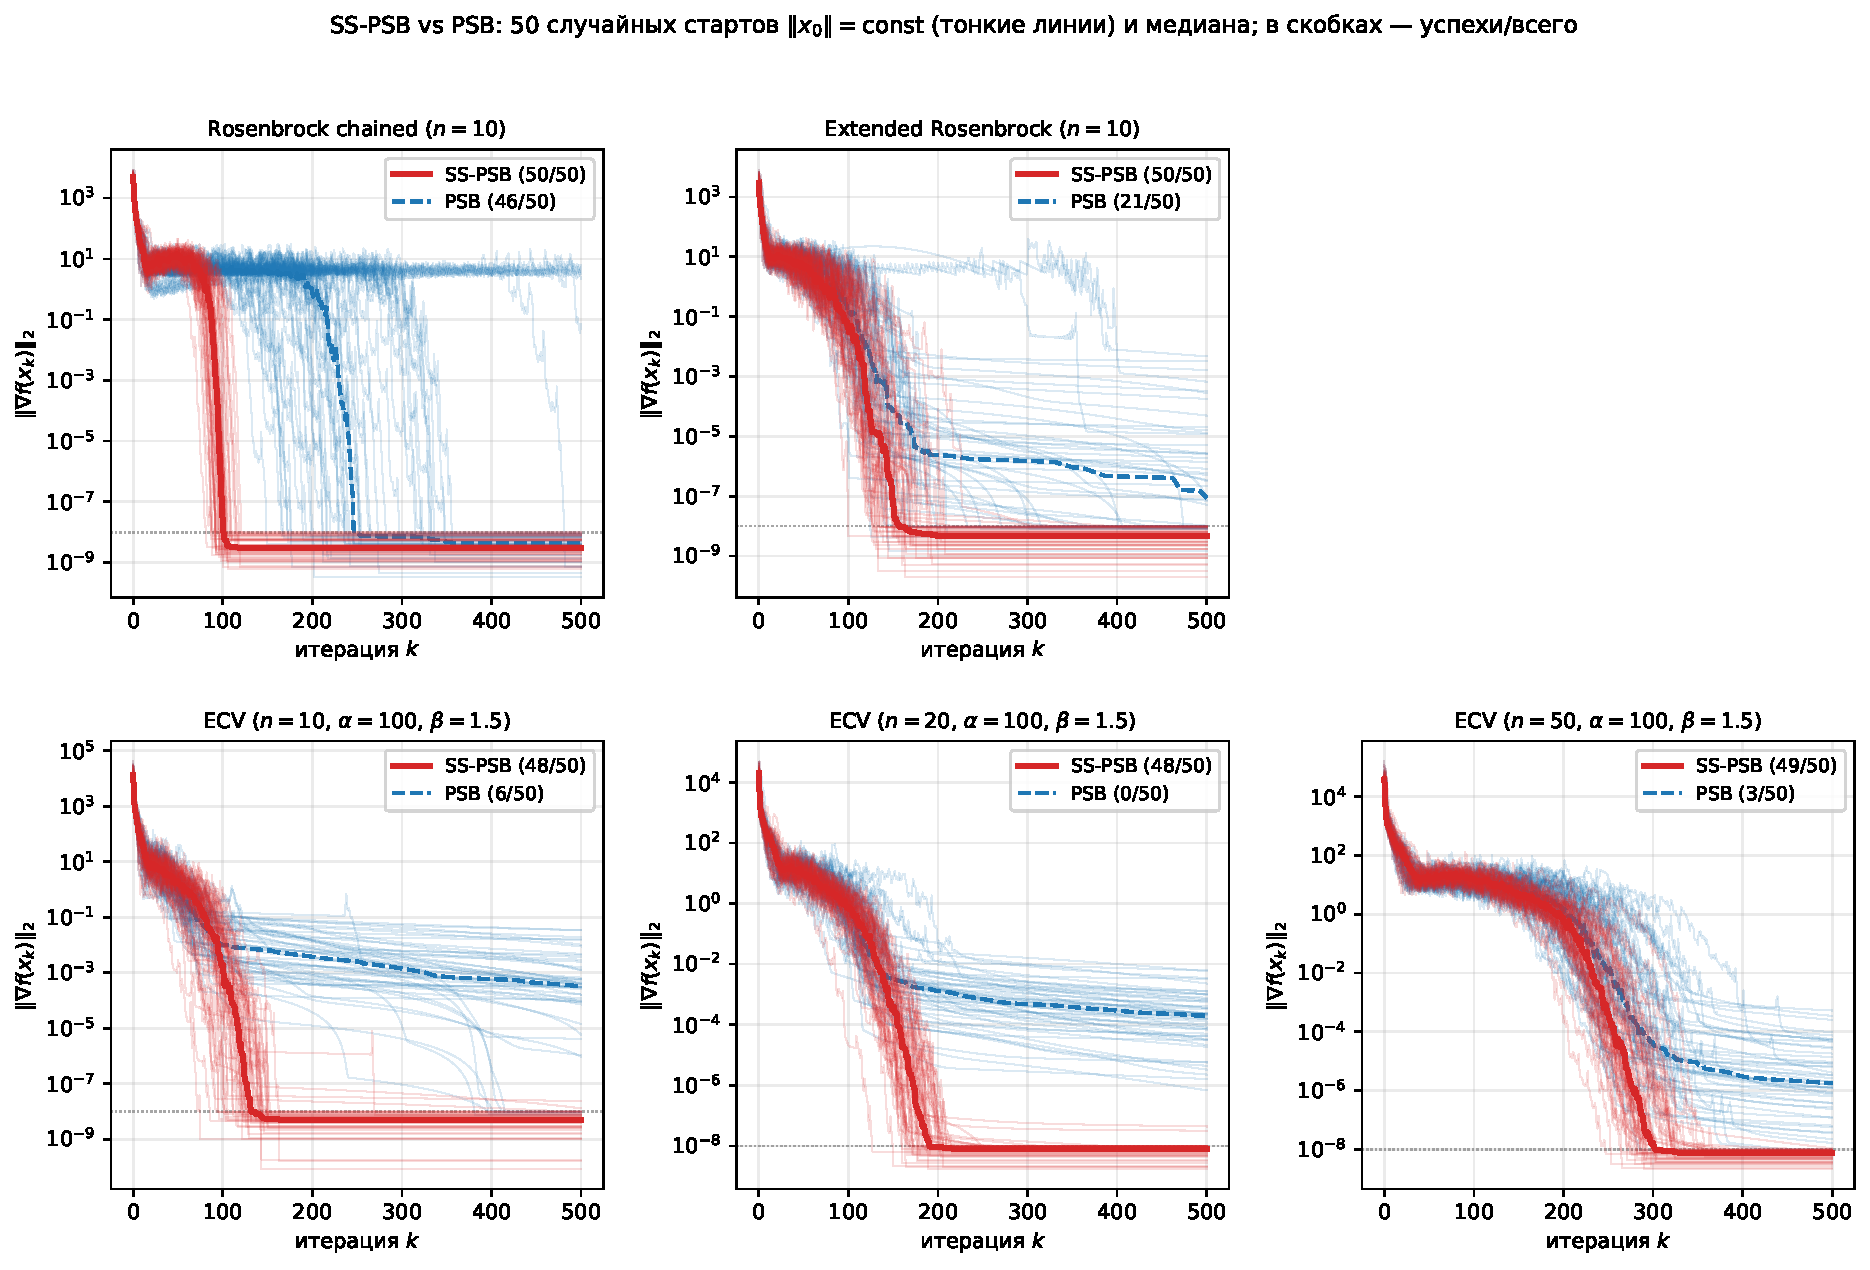
\includegraphics[height=0.60\textheight]{fig_ndim_stat_psb.pdf}
\par\smallskip
{\footnotesize\raggedright
Чистый PSB деградирует (Extended Rosenbrock 21/50; Extended Curved Valley (ECV) —
0--6/50 по трём размерностям \(n=10/20/50\)); SS-PSB устойчиво сходится на всех
конфигурациях (48--50/50). 
SS-коррекция помогает там, где базовое обновление \emph{реально деградирует}; для SR1
со skip-rule деградации нет — и выигрыша SS-SR1 не даёт (зам.~3.17).\par}
\end{frame}

% ===================== ВН (ГЛ.4) =====================
% Говорить ЧЕСТНО про соавторство: VIJI и оценка (82) — совместная [16];
% собственный вклад главы = Утверждение 4.1 (подстановка в δ).
\begin{frame}{Приложение к вариационным неравенствам}
\small
Метод 2-го порядка \textbf{VIJI} для монотонного ВН \(\langle F(x),x-x^*\rangle\ge0\)
использует линейную модель с неточным якобианом \(J(v)\approx\nabla F(v)\); вся
неточность — одно число \(\delta=\nrm{\nabla F(v)-J(v)}\).

\smallskip
\textbf{Скорость (соавторская работа, NeurIPS 2024):}
\[ \mathrm{gap}(\widetilde x_T)=O\!\Big(\tfrac{L_1D^3}{T^{3/2}}+\tfrac{\delta D^2}{T}\Big),
   \qquad\text{зависимость от \(\delta\) неулучшаема.} \]

\smallskip
\textbf{Утверждение 4.1} — \emph{связь} с локальной теорией главы~2
и неточности \(\delta\):
\[ \delta_k=\nrm{B_k-\nabla F(x_k)}\le\Fn{E_k}+L_1\rho_k,\qquad
   \Fn{E_kS_p}=O(\rho_k)\ \text{(следствие 2.12)}. \]

\smallskip
\textbf{Что это даёт:} вместо равномерного потолка \(\delta\le2L_0\) односекущего
L-Broyden — \emph{убывающая} вблизи решения \(\delta_k\): \(\delta\)-член оценки скорости
перестаёт быть постоянным. Улучшение \emph{локальное}; глобального переноса не утверждаем.
\end{frame}

% ===================== ЗАКЛЮЧЕНИЕ =====================
\begin{frame}{Заключение}
\textbf{Результаты.}
{\small
\begin{itemize}
  \item Точное разложение и явная, не зависящая от \(n\) константа bounded deterioration
        для мультисекущего Бройдена; \(O(\rho_k)\)-контроль ошибки на подпространстве.
  \item Limited-memory вариант L-PB, применимый при \(n\sim10^5\).
  \item Симметричный SS-U с условной Q-сверхлинейной сходимостью; эмпирически
        стабилизирует деградирующий PSB.
  \item Локальная оценка ошибки в скорости метода 2-го порядка для ВН.
\end{itemize}}
\textbf{Перспективы.} Формальная глобализация; L-PB на крупномасштабных задачах
(PINN, равновесные модели); замкнутый глобальный вывод для ВН; сравнение с
L-BFGS и Anderson.
\end{frame}

% ===================== СПАСИБО =====================
\begin{frame}[plain,noframenumbering]{}
\vfill
\centering
{\Large Спасибо за внимание!}\par
\vfill
\end{frame}

% ===================== БЭКАП =====================
\appendix

\begin{frame}{Приложение: накопленная невязка прошлых секущих}
\centering
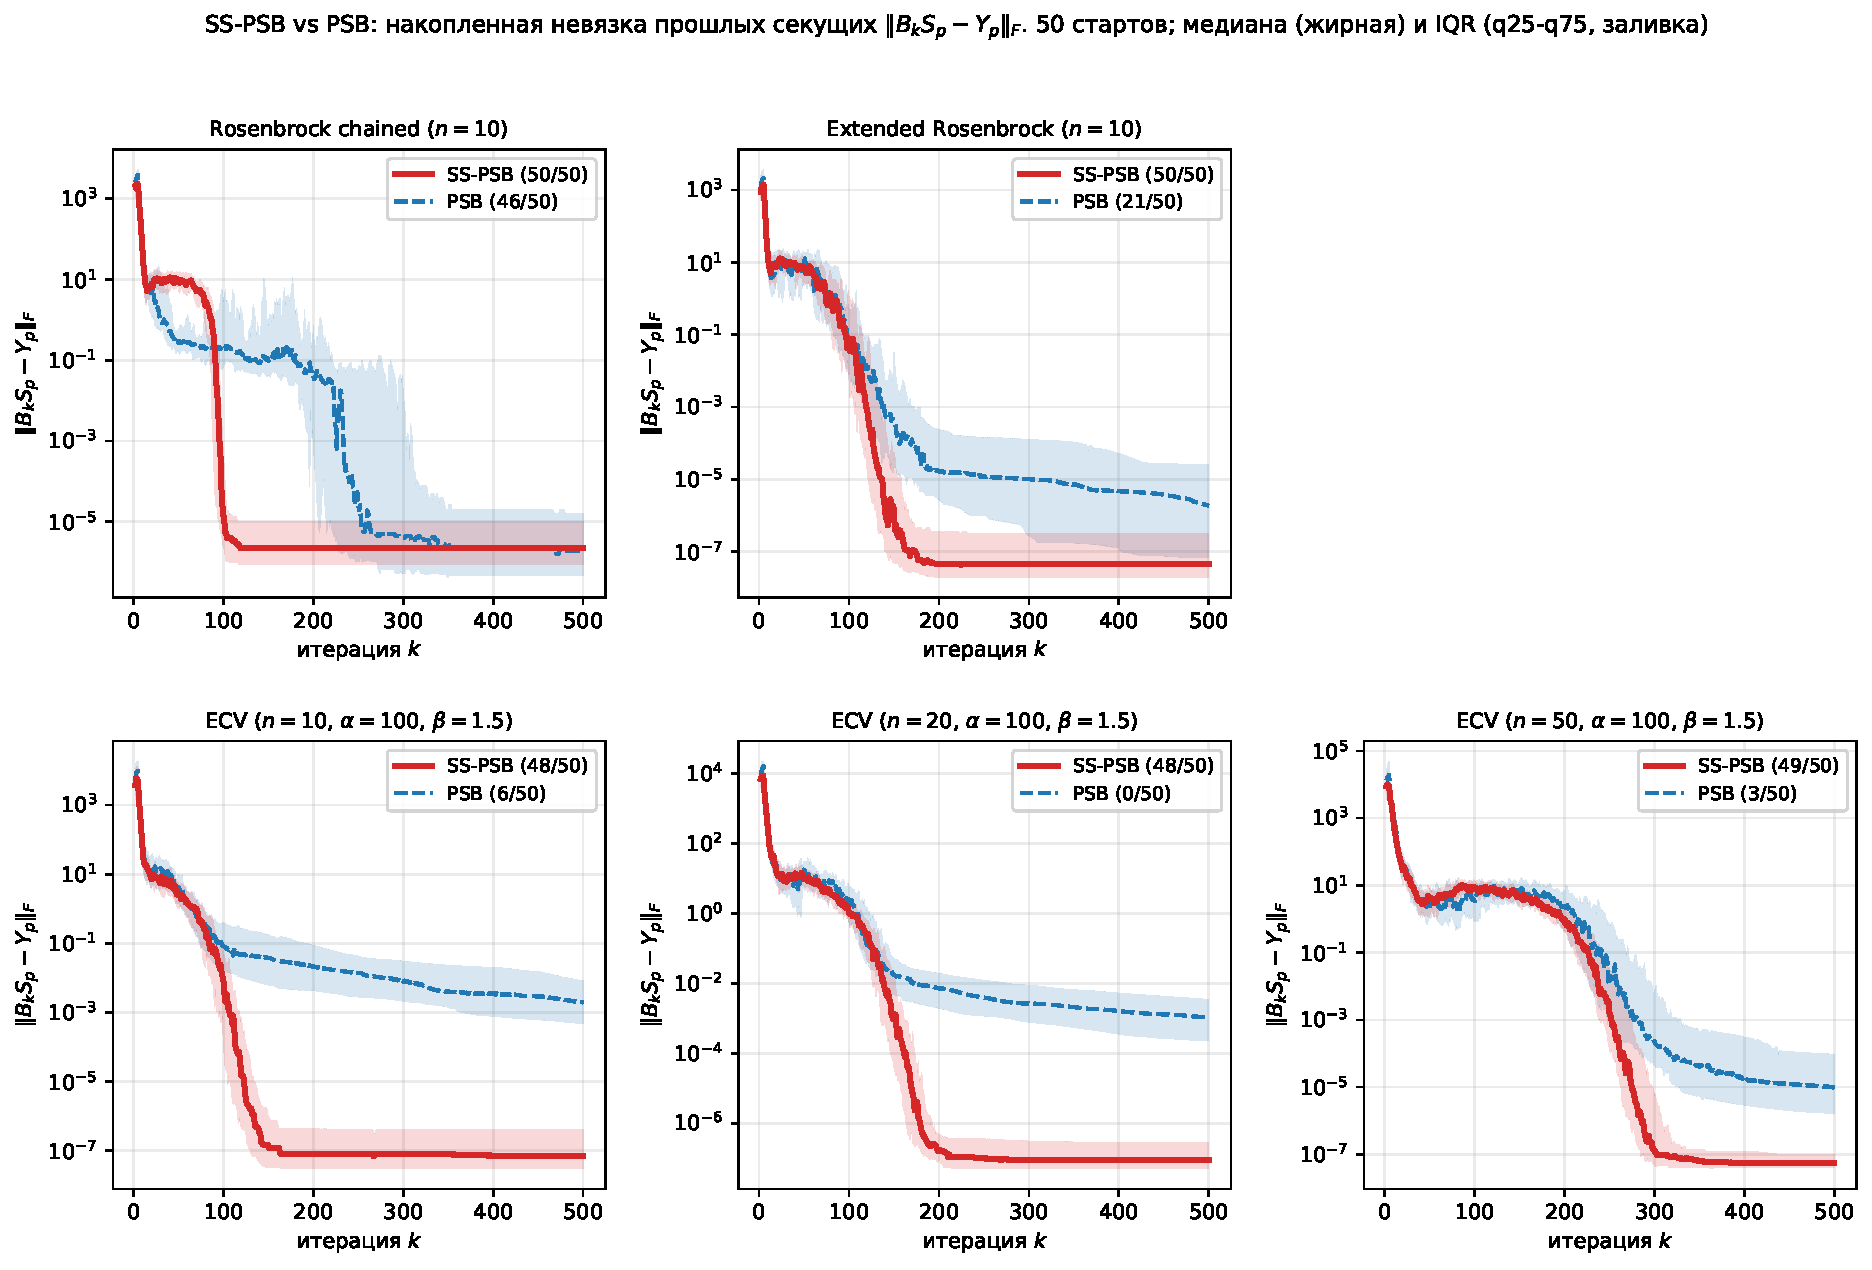
\includegraphics[height=0.62\textheight]{fig_ndim_stat_rpast_psb.pdf}
\par\smallskip
{\footnotesize SS-PSB системно держит \(\Fn{B_kS_p-Y_p}\) ниже PSB — прямое
эмпирическое подтверждение Теоремы 3.8, п.\,3.\par}
\end{frame}

\begin{frame}{Приложение: SS-SR1 vs SR1 (где деградации нет)}
\centering
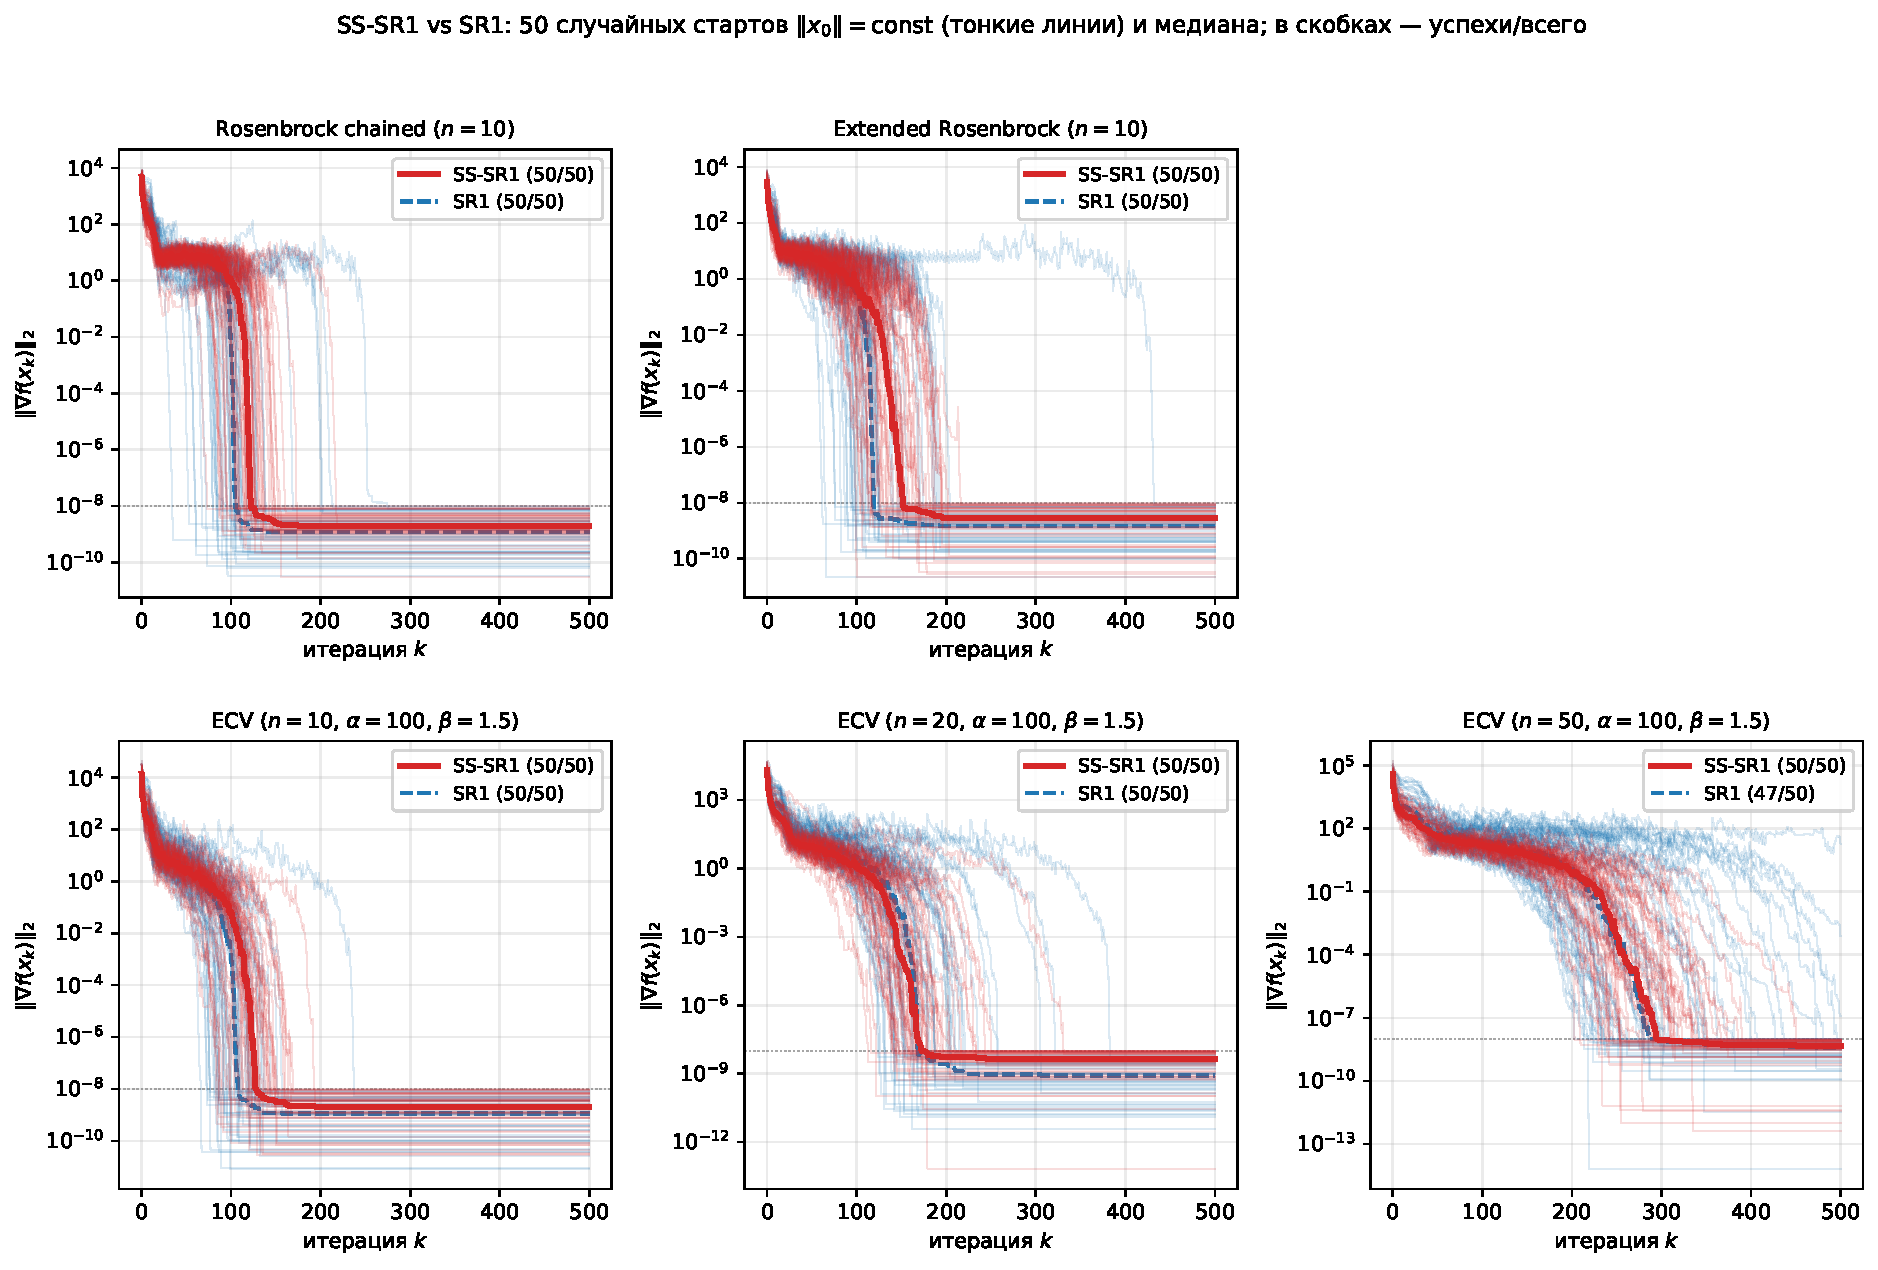
\includegraphics[height=0.60\textheight]{fig_ndim_stat_sr1.pdf}
\par\smallskip
{\footnotesize SR1 со skip-rule не деградирует — SS-коррекция не даёт выигрыша.
\par}
\end{frame}

\begin{frame}{Приложение: роль глобализации (без line search)}
\centering
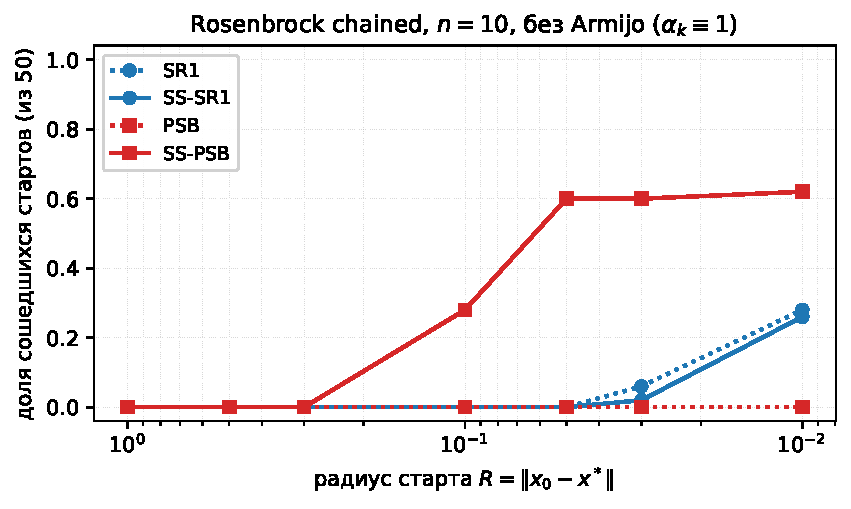
\includegraphics[width=0.60\textwidth]{fig_ss_local_basin.pdf}
\par\smallskip
{\footnotesize Без backtracking полный QN-шаг расходится даже вблизи \(x^*\) на
невыпуклых задачах; SS-коррекция расширяет область устойчивости.\par}
\end{frame}
\end{document}
